\documentclass[10pt,xcolor=dvipsnames]{beamer}
\usepackage[french]{babel}
\usepackage[utf8]{inputenc}
\usepackage[T1]{fontenc}
\usepackage{caption}
\usepackage{algorithm}
\usepackage{algorithmic}
\renewcommand{\algorithmicrequire}{\textbf{Require:}}
\renewcommand{\algorithmicensure}{\textbf{Ensure:}}
\renewcommand{\algorithmiccomment}[1]{\{#1\}}
\renewcommand{\algorithmicend}{\textbf{Fin}}
\renewcommand{\algorithmicif}{\textbf{Si}}
\renewcommand{\algorithmicthen}{\textbf{Alors}}
\renewcommand{\algorithmicelse}{\textbf{Sinon}}
\renewcommand{\algorithmicelsif}{\algorithmicelse\ \algorithmicif}
\renewcommand{\algorithmicendif}{\algorithmicend\ \algorithmicif}
\renewcommand{\algorithmicfor}{\textbf{Pour}}
\renewcommand{\algorithmicforall}{\textbf{Pour tout}}
\renewcommand{\algorithmicdo}{\textbf{faire}}
\renewcommand{\algorithmicendfor}{\algorithmicend\ \algorithmicfor}
\renewcommand{\algorithmicwhile}{\textbf{Tant que}}
\usepackage{MnSymbol,wasysym}
\usepackage{amsmath}
\usepackage{cancel}
\usepackage[draft]{pdfcomment}
\newcommand{\pdfnote}[1]{\marginnote{\pdfcomment[icon=note]{#1}}}
\usepackage{appendixnumberbeamer}
\usepackage{comment}

\renewcommand{\thefootnote}{\fnsymbol{footnote}}




\usetheme[progressbar=frametitle,numbering=fraction]{metropolis}
%LS:
\setbeamercolor{background canvas}{bg=white}  
\usepackage{appendixnumberbeamer}

\usepackage{booktabs}
\usepackage[scale=2]{ccicons}
\usepackage{tikz}
\usepackage{color}
\usepackage{mathtools}

\usetikzlibrary{shapes,snakes}
%% Color Definition
\definecolor{darkspringgreen}{rgb}{0.09, 0.45, 0.27}
\newcommand{\red}[1]{\textcolor{red}{#1}}

\setbeamertemplate{frame footer}{Rohan Fossé}

\setbeamercolor{footline}{fg=gray}

\def\checkmark{\tikz\fill[scale=0.4,color=darkspringgreen](0,.35) -- (.25,0) -- (1,.7) -- (.25,.15) -- cycle;}
\usepackage{pgfplots}
\usepgfplotslibrary{dateplot}

\usepackage{eso-pic}
\usepackage{xspace}
\long\def\/*#1*/{}

\title{
Algorithmique et structure de données
}

\date{\centering 2021-2022}
\author{\centering \bf Rohan Fossé}


\begin{document}

\maketitle



  \begin{frame}{Trivia}

  \textbf{Intervenants}
  \begin{itemize}
 \item Rohan Fossé, \texttt{rfosse@labri.fr}
 \item Jonathan Narboni, \texttt{jnarboni@labri.fr}
  \end{itemize}
 \textbf{Organisation}
  \begin{itemize}
  \item Cours : $6 \times 1h20$
  \item EI :$6\times 2h40$ 
  \item TP : $5 \times 1h20$ 
    % \item \sout{\textbf{Examen} : le \textbf{lundi 24 novembre 2014 }} reporté
  \end{itemize}
  \textbf{Modalités de contrôle}
  \begin{itemize}
      \item Examen écrit \underline{sans document}: 2h
  \end{itemize}
  
  \end{frame}
  
  \begin{frame}{Objectifs de l'UE}
      \begin{itemize}
          \item Se familiariser avec des problèmes classiques et leur solutions;
          \item Se préparer à trouver des solutions algorithmiques à des problèmes en sachant comparer leurs performances;
          \item S'entraîner à écrire des algorithmes et connaître les différentes structures de données.
      \end{itemize}
  \end{frame}

\section{Introduction}
%=========================================================
%=========================================================
\begin{frame}{Algorithmique et Structures de Données}
  \begin{itemize}
  \item \textbf{Algorithme}  : séquence d'opérations de calcul élémentaires, organisé selon des règles précises dans le but de résoudre un problème donné.
  \item \textbf{Structures de données} : moyen de stocker et organiser des données pour faciliter l'accès à ces données et leur modification.
  \end{itemize}
\end{frame}

\begin{frame}
  \begin{center}
    {\alert{\huge{Algorithmes}}}
  \end{center}
\end{frame}

\begin{frame}{Exemple d'algorithme}
\begin{alertblock}{Boire son café}
\begin{enumerate}[<+->]
    \item Prenez une dosette de café.
    \item Mettez-la dans la machine à café.
    \item  Vérifiez si la machine à café est allumée. Si ce n'est pas le cas, allumez la machine.
    \item  Vérifiez si le filtre à eau est suffisamment rempli. - Si ce n'est pas le cas, ajoutez de l'eau.
    \item Placez une tasse à café sous le distributeur de café.
    \item Appuyez sur le bouton café.
    \item Le café est en train d'être servi. - Attendez que la machine indique que le café est prêt.
    \item Si le café est prêt - Sortez la tasse à café de la machine à café.
\end{enumerate}
\end{alertblock}

\end{frame}


\begin{frame}{Autre exemple d'algorithme}
\begin{alertblock}{Se laver les mains}
\begin{enumerate}[<+->]
\item Ouvrir l'eau
\item Mettre du savon
\item Nettoyer ses mains avec l'eau
\item Éteindre l'eau
\item Se sécher les mains
\end{enumerate}
\end{alertblock}
\begin{center}
\only<6>{
\alert{Qu'est ce qu'un algorithme ?}
}
\end{center}
\end{frame}

\begin{frame}{Un algorithme}
    \begin{itemize}
        \item Un algorithme est une méthode systématique (comme une recette) pour résoudre un problème donné;
        \item Il se compose d'une suite d'opérations simples à effectuer pour résoudre ce problème;
        \item En informatique, \textbf{cette méthode doit être applicable par un ordinateur}.
    \end{itemize}
\end{frame}

\begin{frame}{Importance de l'algorithmique}
    \begin{itemize}
        \item Pour un problème donné, il existe plusieurs algorithmes;
        \item Il est facile d'écrire des algorithmes faux ou inefficaces;
        \item Une erreur peut faire la différence entre quelques minutes de calculs et plusieurs heures;
        \item C'est souvent une question d'utilisation de structures de données ou d'algorithmes connus dans la littérature.
    \end{itemize}
\end{frame}


 
\begin{frame}{Exemple: la ville et la pizzeria}

    \begin{exampleblock}{Le problème}
    Nous allons considérer 3 villes contenant 14 maisons et 1 pizzeria. Nous souhaitons savoir quelle ville permet aux livreurs de pizza de faire les trajets les plus rapides et pourquoi.
    \end{exampleblock}

    \begin{figure}
        \centering
        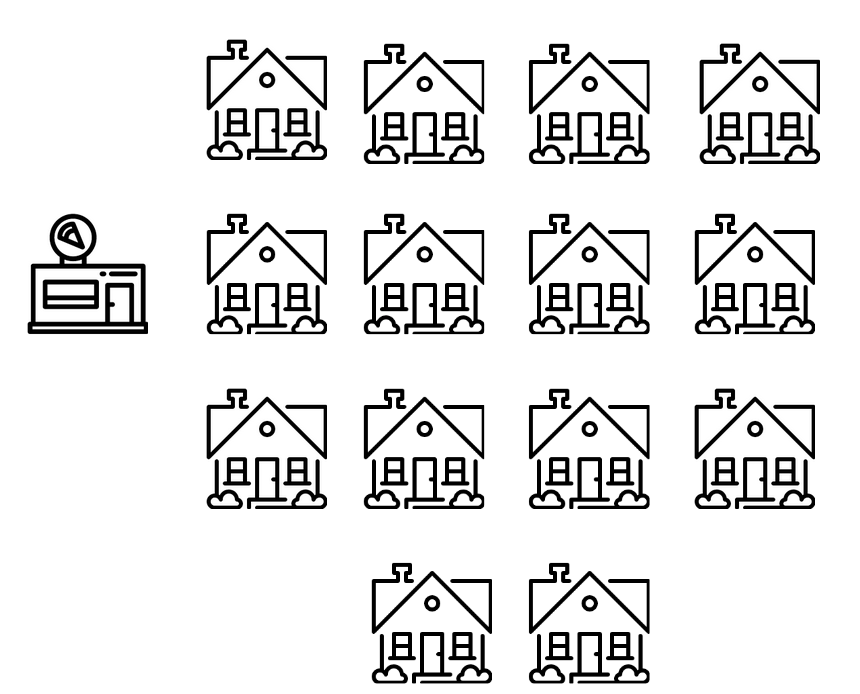
\includegraphics[scale=0.17]{figures/CM0/Pizzeria-1.png}
        \caption{1 pizzeria et 14 maisons}
        \label{fig:piz2}
    \end{figure}
\end{frame}

\begin{frame}{Exemple: la ville et la pizzeria}

    \begin{exampleblock}{Le problème}
    Nous allons considérer 3 villes contenant 14 maisons et 1 pizzeria. Nous souhaitons savoir quelle ville permet aux livreurs de pizza de faire les trajets les plus rapides et pourquoi.
    \end{exampleblock}

    \begin{alertblock}{Temps de calcul}
    On suppose qu'il faut une \alert{unité de temps} pour passer d'une maison à un autre, en suivant une rue.
    \end{alertblock}
    \only<1->{\vspace{-0.3cm}
    \begin{figure}
        \centering
        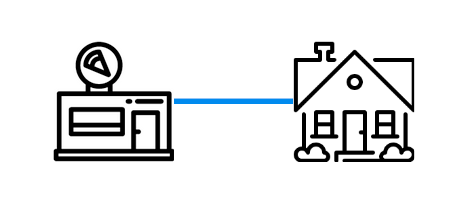
\includegraphics[scale=0.35]{figures/CM0/Pizzeria-Maison.png} 
        \vspace{-0.6cm}
        \caption{Trajet entre la pizzeria et une maison}
    \end{figure}
    }
    \begin{center}
    \uncover<2>{
        \alert{Dans le pire cas, quel est le temps mis par un livreur pour aller de la pizzeria jusqu'à une maison ?}
    }
    \end{center}
\end{frame}


\begin{frame}{Ville A}
\begin{exampleblock}{Organisation de la ville}
Les maisons sont rangées dans l'ordre croissant en ligne droite. La pizzeria se trouve au numéro 1.
\end{exampleblock}
\uncover<2->{
    \begin{figure}
        \centering
        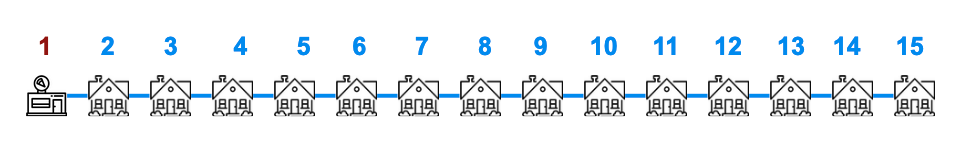
\includegraphics[scale=0.30]{figures/CM0/Pizzeria-2.png}

        \label{fig:piz2}
    \end{figure}
}
\uncover<3->{
    \begin{center}
        Quel est le pire temps possible? \only<4>{\textbf{14}}
    \end{center}
 }  
    
\end{frame}

\begin{frame}{Ville B}
\begin{exampleblock}{Organisation de la ville}
Même organisation que dans la ville A, mais cette fois-ci la pizzeria est au numéro \textbf{8}
\end{exampleblock}
\uncover<2->{
    \begin{figure}
        \centering
        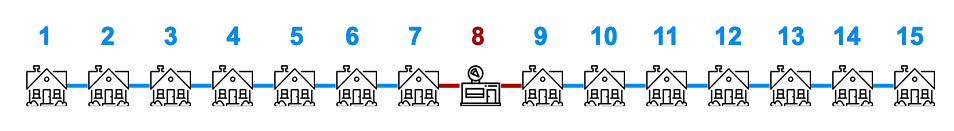
\includegraphics[scale=0.30]{figures/CM0/Pizzeria-3.png}

        \label{fig:piz2}
    \end{figure}
}
\uncover<3->{
    \begin{center}
        Quel est le pire temps possible? \only<4>{\textbf{7}}
    \end{center}
 }  
    
\end{frame}

\begin{frame}{Ville C}
\begin{exampleblock}{Organisation de la ville}
Cette fois-ci, les maisons sont organisées en embranchements, la pizzeria est tout en \textbf{haut}.
\end{exampleblock}
        \begin{figure}
        \centering
        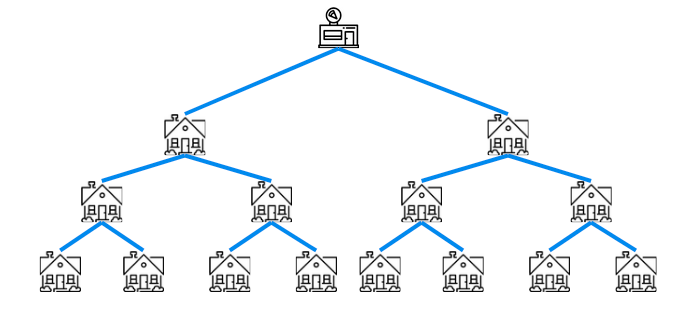
\includegraphics[scale=0.40]{figures/CM0/Pizzeria-4.png}

        \label{fig:piz4}
    \end{figure}
    
    \begin{center}
        \uncover<1-2>{Quel est le pire temps possible? \only<2>{\textbf{3}}}
        \uncover<3>{
        \alert{Comment numéroter les maisons ?}
        }
    \end{center}
\end{frame}

\begin{frame}{Ville C : première numérotation}
        \begin{figure}
        \centering
        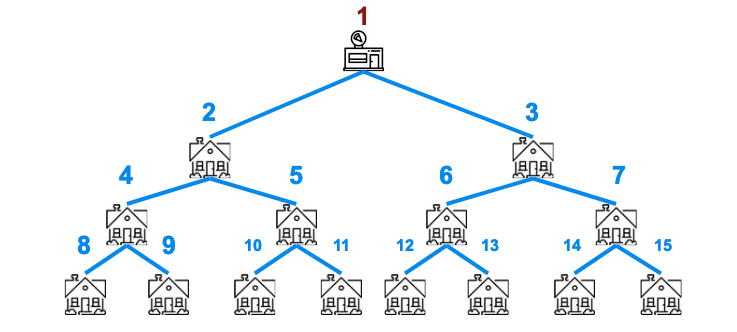
\includegraphics[scale=0.40]{figures/CM0/Pizzeria-5.png}

        \label{fig:piz5}
    \end{figure}
    
    \begin{center}
        \uncover<2>{
        \alert{Comment choisir la bonne rue à prendre ?}
        }
        
    \end{center}
\end{frame}

\begin{frame}{Ville C : deuxième numérotation}
        \begin{figure}
        \centering
        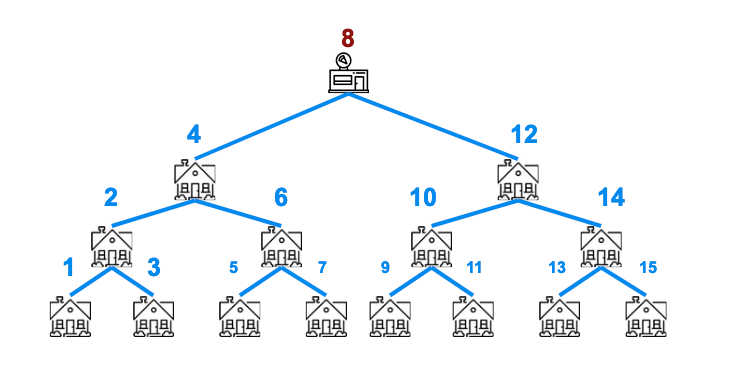
\includegraphics[scale=0.40]{figures/CM0/Pizzeria-6.png}

        \label{fig:piz6}
    \end{figure}
    
    \uncover<2>{
    \begin{center}
        Dans ce cas là, si le numéro de la maison à livrer est plus petit que celui sur lequel on se trouve, on va à gauche, sinon on va à droite.
    \end{center}
    }
\end{frame}


\begin{frame}{Tableau récapitulatif}
    \begin{table}[]
\begin{tabular}{|c|c|c|c|}
\hline
\textbf{Nombre de maisons} &\textbf{Ville A} & \textbf{Ville B} & \textbf{Ville C} \\ \hline
\textbf{15}                & 14                                       & 7                                        & 3                                        \\ \hline
\uncover<2->{\textbf{1023}              &} \uncover<3->{1022                                     & 511                                      & 9                                        \\ \hline}
\uncover<4->{\textbf{n}                 &} \uncover<5->{n-1                                      &} \uncover<6->{$\frac{n-1}{2}$                                  &} \uncover<7->{$\approx log_2(n)$                                 \\ \hline}
\end{tabular}
\end{table}

\end{frame}

\begin{frame}{Et pourquoi pas en étoile ?}
        \begin{figure}
        \centering
        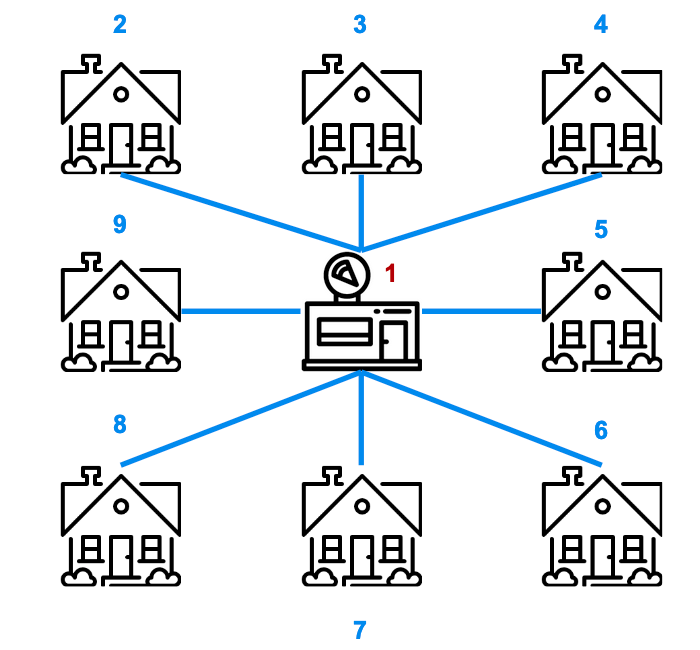
\includegraphics[scale=0.25]{figures/CM0/Pizzeria-etoile.png}

        \label{fig:piz6}
    \end{figure}
    
    \begin{center}
        \only<1>{Cette configuration semble optimale, quel peut être le problème ?}
        \only<2>{Une organisation en étoile avec la pizzeria au milieu permet des trajets très courts, mais \alert{choisir} la bonne rue prend du temps.}
    \end{center}
\end{frame}

\begin{frame}{Complexité: quelques définitions}

\begin{alertblock}{Complexité}
La \textbf{\alert{complexité}} dans le pire cas d'un algorithme est la fonction mathématique $\mathcal{T}$ qui donne le \alert{nombre maximal d'instructions élémentaires} que l'algorithme effectue en fonction de la taille des données manipulées.\\
\end{alertblock}

\begin{exampleblock}{Exemple précédent}
Dans notre exemple précédent, la taille des données manipulées étaient le nombre de maisons.
\end{exampleblock}
\end{frame}

\begin{frame}{Complexité dans le pire cas: A quoi ça sert ?}
    \begin{itemize}
        \item \alert{\textbf{Évaluer le temps d'exécution}} d'un algorithme en fonction de la longueur de l'énoncé;
        \item \alert{\textbf{Comparer les performances}} de différents algorithmes résolvant le même problème;
        \item \alert{\textbf{Évaluer la taille maximale}} des énoncés qu'un algorithme peut traiter;
        \item Mesure du temps \alert{\textbf{indépendante des machines}} puisque l'on compte le nombre d'instructions.
    \end{itemize}
\end{frame}


\begin{frame}{Ordre de grandeur}
Pour comparer des algorithmes, il n'est pas nécessaire d'utiliser la fonction $\mathcal{T}$, mais seulement l'ordre de grandeur asymptotique, noté $\mathcal{O}$ (prononcé "\textit{grand O}").

\begin{alertblock}{Définition formelle}
Une fonction $\mathcal{T}(n)$ est en $\mathcal{O}(f(n))$ ("\textit{en grand O de f(n)}") si:
\begin{equation*}
    \exists n_o \in \mathbb{N}, \exists c \in \mathbb{R}^+, \forall n \in \mathbb{R}^+, n \geq n_0 \implies | T(n) | \leq c | f(n) | 
\end{equation*}
\end{alertblock}

\only<1>{
Autrement dit, $\mathcal{T}(n)$ est en $\mathcal{O}(f(n))$ s'il existe un seuil $n_0$ à partir duquel la fonction $\mathcal{T}$ est toujours dominée par la fonction $f$, à une constance multiplicative fixée $c$.
}

\end{frame}


\begin{frame}{Quelques exemples}
    \begin{exampleblock}{Exemples}
\begin{itemize}
    \item $T_1(n) = 7 \only<2->{= \mathcal{O}(7)} = \only<3->{\mathcal{O}(1)}$
    \item $T_2(n) = 12n + 5 \only<4->{= \mathcal{O}(12n)} \only<5->{= \mathcal{O}(n)}$
    \item $T_3(n) = 4n^2 + 2n + 6 \only<6->{= \mathcal{O}(4n^2 + 2n)} \only<7->{= \mathcal{O}(n^2)}$
    \item $T_4(n) = 2 + (n-1) \times 5 \only<8->{= \mathcal{O}(n-1)} \only<9->{= \mathcal{O}(n)}$
\end{itemize}
\end{exampleblock}

\uncover<10->{
\begin{exampleblock}{A vous de jouer}
Quelle est la complexité dans le pire des cas des exemples suivants ?
\begin{itemize}
    \item $T_5(n) = 3n + log(n)^4 + 2 \only<11->{= \mathcal{O}(n)}$
    \item $T_6(n) = 1024  \only<12->{= \mathcal{O}(1)}$
    \item $T_7(n) = 2^n + n^{10} \only<13->{= \mathcal{O}(2^n)}$
\end{itemize}
\end{exampleblock}
}

\end{frame}

\begin{frame}{Rappels des règles utiles}
Les quelques règles suivantes permettent de simplifier les complexités en omettant des termes dominés :
\begin{itemize}
    \item Les \alert{coefficients peuvent être omis} : $14n^2$ devient $n^2$;
    \item $n^a$ domine $n^b$ si $a > b$ : par exemple, $n^2$ domine $n$;
    \item Une exponentielle domine un polynôme : $3^n=exp^{nlog 3}$ domine $n^5$;
    \item De même un polynôme domine un logarithme : n domine $(log n)^3$. Cela signifie également que, par exemple, $n^2$ domine $n log n$.
\end{itemize}
\end{frame}



\begin{frame}{Reprenons notre pizzeria}

\begin{table}[]
\begin{tabular}{|c|c|c|c|}
\hline
\textbf{Nombre de maisons} &\textbf{Ville A} & \textbf{Ville B} & \textbf{Ville C} \\ \hline
\textbf{15}                & 14                                       & 7                                        & 3                                        \\ \hline
\textbf{1023}              & 1022                                     & 511                                      & 9                                        \\ \hline
\textbf{n}                 & n-1                                      & $\frac{n-1}{2}$                                  & $log_2(n)$                                 \\ \hline

\only<2->{
\red{\textbf{Complexité pour n}}              & \red{$\mathcal{O}(n)$}                                     & \red{$\mathcal{O}(n)$}                                       & \red{$\mathcal{O}(log(n))$ }                                        \\ \hline
}
\end{tabular}
\end{table}   
\begin{center}
    \uncover<3->{
        On voit que les complexités dans le pire cas de la ville A et de la ville B \textbf{sont les mêmes}
    }
\end{center}
\end{frame}

\begin{frame}{Reprenons notre exemple}
    \begin{itemize}
        \item Dans la ville A et B, l'algorithme naturel pour trouver une maison a une complexité linéaire $\mathcal{O}(n)$
        \item Dans la ville C, l'algorithme naturel pour trouver une maison a une complexité logarithmique $\mathcal{O}(log(n))$
        \item L'organisation de la ville C est beaucoup plus efficace pour livrer les pizzas.
    \end{itemize}
    \uncover<2->{
    \begin{center}
        \alert{À quel point est-ce que c'est plus efficace ?}
    \end{center}
    }
\end{frame}

\begin{frame}{Différence entre n et log n}
    \begin{figure}
        \centering
        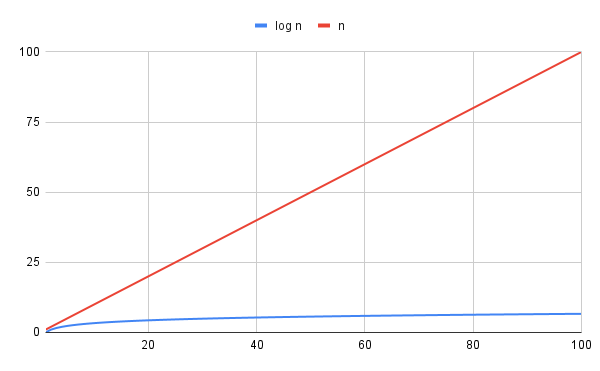
\includegraphics[scale=0.4]{figures/CM0/comp_n_log_n.png}
    \end{figure}
    \begin{itemize}
        \item Si $n = 10^6$, alors $log_2(n) \approx 20 $. Le livreur fait 50 000 fois moins de déplacements si les maisons sont organisées comme dans la ville C.
        
    \end{itemize}
\end{frame}

\begin{frame}{Classe de complexité}
\begin{table}[]
\centering
\begin{tabular}{|c|c|c|c|}
\hline
\textbf{Complexité} & \textbf{Notation}\\
\hline
constante & $\mathcal{O}(1)$ \\
logarithmique &   $\mathcal{O}(log(n))$\\
racinaire &   $\mathcal{O}(\sqrt{x})$ \\
linéaire &    $\mathcal{O}(n)$ \\
quasi-linéaire & $\mathcal{O}(nlog(n))$ \\
quadratique (polynomial) &     $\mathcal{O}(n^2)$ \\
cubique (polynomial) &   $\mathcal{O}(n^3)$ \\
sous-exponentielle &   $\mathcal{O}(2^{poly(log(n))})$ \\
exponentielle &    $\mathcal{O}(2^{poly(n)})$ )\\
factorielle &  $\mathcal{O}(n!)$\\
\hline
\end{tabular}
\captionsetup{justification=centering}
\caption{Évolution du temps de calcul en fonction de la complexité d'un algorithme et de la taille des données}
\label{table:Complexity}
\end{table}

\end{frame}

\begin{frame}{Il existe d'autres complexités}
    \begin{alertblock}{Complexité en moyenne}
    \begin{itemize}
        \item Il s'agit de la complexité en moyenne sur toutes les entrées;
        \item Intéressant car certains problèmes ont une complexité dans le pire cas très élevées, mais les entrées qui correspondent à ces cas ne se produisent que très rarement en pratique;
        \item Étudié essentiellement dans les algorithmes de tri (que nous verrons plus tard)
    \end{itemize}
    \end{alertblock}
    
        \begin{alertblock}{Complexité en mémoire}
    \begin{itemize}
        \item On souhaite ici mesurer la mémoire utilisée par un algorithme;
        \item Certains algorithmes sont en effet très rapide mais prennent beaucoup d'espace mémoire (ou inversement);
    \end{itemize}
    \end{alertblock}
    
    \begin{center}
        Il existe plusieurs autres complexités mais qui ne nous concernent pas directement.
    \end{center}
\end{frame}

\section{Langage de Description Algorithmique}


\begin{frame}{Plus grand diviseur commun (pgcd)}
  \underline{Problème}:
  \begin{itemize}
  \item Entrées: 2 entiers $a>b \geq 0$
  \item Sortie: le  pgcd de $\mathbf{a}$ et $\mathbf{b}$
  \end{itemize}
  Exemple: $     pgcd(123,82) = 41$  \\~\\
  ~\\\uncover<2->{\underline{Opérations élémentaires}: $+,\times,-$ et division euclidienne\\~\\}
  
  \uncover<3->{$
    \noindent\underline{\mbox{Observation}}: \left\{
      \begin{array}{ll}
        pgcd(a,b) & =  pgcd(b,r)  \ \ \mbox{r reste de la div. de a par b} \\
        pgcd(a,0) & = a
      \end{array} \right.
  $
  ~\\~\\Exemple: $pgcd(123,82) = pgcd(82,41) = pgcd(41,0) = 41$}
\end{frame}

\begin{frame}{Pgcd: écriture d' un algorithme}
  $\noindent\underline{\mbox{Observation}}: \left\{
      \begin{array}{ll}
        pgcd(a,b) & =  pgcd(b,r) \ \ \mbox{r reste de la div. de a par b}\\
        pgcd(a,0) & = a \\
      \end{array} \right.
  $\\
\underline{Algorithme}: \only<1>{???}
\begin{tabbing}
  aaa\=aaa\=\kill
  \only<9->{\textbf{pgcd}(a,b) \hfill $~~~~~~~~~~~~~~~~~~$\texttt{/* a,b entiers, $a>b \geq 0$ */}}  \\
  \> \only<2->{ \textbf{si} $b=0$ \textbf{retourner} $a$ \textbf{fin si}} \\
  \> \only<3->{ $x \leftarrow a; y \leftarrow b$} \\
  \> \only<6->{\textsl{répéter}} \\
  \> \> \only<3->{$r \leftarrow$ reste de la div. euclidienne de $x$ par $y$} \\
  \> \> \only<4->{\textbf{si} $r = 0$ \textbf{alors} \textbf{retourner} $y$} \\
  \> \> \only<5->{\textbf{sinon} $x \leftarrow y$; $y\leftarrow r$} \\
  \> \> \only<5->{\textbf{fin si}} \\
  \> \only<6->{\textsl{fin répéter}} 
  \end{tabbing}
\end{frame}

\begin{frame}{Algorithme d'Euclide}
  \begin{minipage}{0.45\linewidth}
    \begin{tabbing}
      aaa\=aaa\=\kill
      \textbf{pgcd}(a,b) \\%\hfill $~~~~~~~~~~~~~~~~~~$\texttt{/* a,b entiers, $a>b \geq 0$ */}  \\
      \>  entier $x,y,r$  \\
 \> \only<2->{ \textbf{si} $b=0$ \textbf{retourner} $a$ \textbf{fin si}} \\
      \> \only<2>{$\red{\mathbf{x \leftarrow a; y \leftarrow b}}$} \only<1,3->{$x \leftarrow a; y \leftarrow b$} \\ 
      \> \textbf{tant que} \only<1-17,19->{$y \neq 0$}\only<18>{$\red{\mathbf{y \neq 0}}$} \textbf{faire} \\
       \> \> \only<3,6,9,12,15>{$\red{\mathbf{r\leftarrow x ~\%~ y}}$} \only<1-2,4-5,7-8,10-11,13-14,16->{$r \leftarrow x ~\%~ y$} \\
       \> \> \only<4,7,10,13,16>{$\red{\mathbf{x \leftarrow y}}$}      \only<1-3,5-6,8-9,11-12,14-15,17->{$x \leftarrow y$}\\
       \> \> \only<5,8,11,14,17>{$\red{\mathbf{y\leftarrow r}}$}       \only<1-4,6-7,9-10,12-13,14-15,18->{$y \leftarrow r$}\\
       \> \textbf{fin tant que} \\
      \> \only<1-18>{\textbf{retourner}($x$)}\only<19>{\red{\textbf{retourner}}($\red{\mathbf{x}}$)}
    \end{tabbing}
  \end{minipage}\hfill
  \begin{minipage}{0.45\linewidth}
    \textbf{pgcd}(12345678,123456) \\
     \begin{tabular}{l|l|l}
       r & x & y \\
       \hline
       \only<2->{$\bot$} & \only<2->{12345678}   & \only<2->{123456} \\
       \only<3->{78} 	 & \only<4->{123456} 	 & \only<5->{78} \\
       \only<6->{60} 	 & \only<7->{78} 	 & \only<8->{60} \\
       \only<9->{18} 	 & \only<10->{60} 	 & \only<11->{18} \\
       \only<12->{6} 	 & \only<13->{18} 	 & \only<14->{6} \\ 
       \only<15->{0} 	 & \only<16-18>{6}\only<19>{\red{\textbf{6}}} 	 & \only<17->{0} \\
       \end{tabular}
\end{minipage}
\end{frame}



\end{document}

